\documentclass{standalone}
\usepackage{tikz}
\definecolor{applegreen}{rgb}{0.55, 0.71, 0.0}
\definecolor{airforceblue}{rgb}{0.36, 0.54, 0.66}
\definecolor{amber}{rgb}{1.0, 0.49, 0.0}
\begin{document}
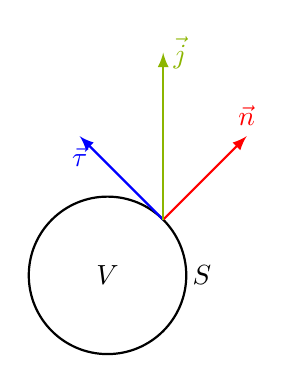
\begin{tikzpicture}
    % Dibujar el círculo
    \draw[thick] (0,0) circle(1); % Círculo de radio 1 cm

    % Etiquetas para V y S
    \node at (0,0) {$V$}; % Etiqueta en el interior del círculo
    \node at (1.2, 0) {$S$}; % Etiqueta en el contorno del círculo
    

    % Vector normal a 45 grados del polo norte
    \draw[-latex, thick, red] ({cos(45)},{sin(45)}) -- ({cos(45)+1.5*cos(45)},{sin(45)+1.5*sin(45)}) node[anchor=south] {$\vec{n}$};

    % Vector tangencial perpendicular apuntando hacia abajo
    \draw[-latex, thick, blue] ({cos(45)},{sin(45)}) -- ({cos(45)-1.5*sin(45)},{sin(45)+1.5*cos(45)}) node[anchor=north] {$\vec{\tau}$};

    % Vector suma \vec{j} que es la suma de \vec{n} + \vec{\tau}
    \draw[-latex, thick, applegreen] ({cos(45)},{sin(45)}) -- ({cos(45)+1.5*(cos(45)-sin(45))},{sin(45)+1.5*(sin(45)+cos(45))}) node[anchor=west] {$\vec{j}$};

\end{tikzpicture}
\end{document}